\begin{equation}
    \begin{gathered}
        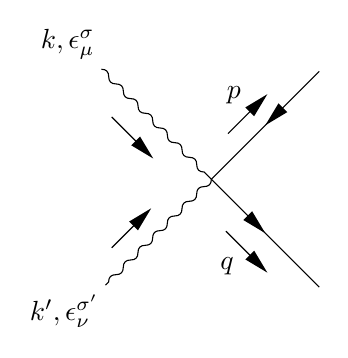
\begin{tikzpicture}[x=0.75pt,y=0.75pt,yscale=-1,xscale=1]
            %uncomment if require: \path (0,300); %set diagram left start at 0, and has height of 300
            
            %Straight Lines [id:da21978589206393995] 
            \draw    (111,112) .. controls (113.36,112) and (114.54,113.18) .. (114.54,115.54) .. controls (114.54,117.89) and (115.72,119.07) .. (118.07,119.07) .. controls (120.43,119.07) and (121.61,120.25) .. (121.61,122.61) .. controls (121.61,124.96) and (122.79,126.14) .. (125.14,126.14) .. controls (127.5,126.14) and (128.68,127.32) .. (128.68,129.68) .. controls (128.68,132.03) and (129.86,133.21) .. (132.21,133.21) .. controls (134.57,133.21) and (135.75,134.39) .. (135.75,136.75) .. controls (135.75,139.1) and (136.93,140.28) .. (139.28,140.28) .. controls (141.64,140.28) and (142.82,141.46) .. (142.82,143.82) .. controls (142.82,146.18) and (144,147.36) .. (146.36,147.36) .. controls (148.71,147.36) and (149.89,148.54) .. (149.89,150.89) .. controls (149.89,153.25) and (151.07,154.43) .. (153.43,154.43) .. controls (155.78,154.43) and (156.96,155.61) .. (156.96,157.96) .. controls (156.96,160.32) and (158.14,161.5) .. (160.5,161.5) -- (164,165) -- (164,165) ;
            %Straight Lines [id:da9856052975518923] 
            \draw    (164,165) .. controls (164,167.36) and (162.82,168.54) .. (160.46,168.54) .. controls (158.11,168.54) and (156.93,169.72) .. (156.93,172.07) .. controls (156.93,174.43) and (155.75,175.61) .. (153.39,175.61) .. controls (151.04,175.61) and (149.86,176.79) .. (149.86,179.14) .. controls (149.86,181.5) and (148.68,182.68) .. (146.32,182.68) .. controls (143.97,182.68) and (142.79,183.86) .. (142.79,186.21) .. controls (142.79,188.57) and (141.61,189.75) .. (139.25,189.75) .. controls (136.9,189.75) and (135.72,190.93) .. (135.72,193.28) .. controls (135.72,195.64) and (134.54,196.82) .. (132.18,196.82) .. controls (129.82,196.82) and (128.64,198) .. (128.64,200.36) .. controls (128.64,202.71) and (127.46,203.89) .. (125.11,203.89) .. controls (122.75,203.89) and (121.57,205.07) .. (121.57,207.43) .. controls (121.57,209.78) and (120.39,210.96) .. (118.04,210.96) .. controls (115.68,210.96) and (114.5,212.14) .. (114.5,214.5) -- (113,216) -- (113,216) ;
            %Straight Lines [id:da9772050670458003] 
            \draw    (164,165) -- (216,217) ;
            \draw [shift={(190,191)}, rotate = 225] [fill={rgb, 255:red, 0; green, 0; blue, 0 }  ][line width=0.08]  [draw opacity=0] (12,-3) -- (0,0) -- (12,3) -- cycle    ;
            %Straight Lines [id:da4232647913189236] 
            \draw    (216,113) -- (164,165) ;
            \draw [shift={(190,139)}, rotate = 315] [fill={rgb, 255:red, 0; green, 0; blue, 0 }  ][line width=0.08]  [draw opacity=0] (12,-3) -- (0,0) -- (12,3) -- cycle    ;
            %Straight Lines [id:da02356337350673887] 
            \draw    (171,190) -- (189.59,208.59) ;
            \draw [shift={(191,210)}, rotate = 225] [fill={rgb, 255:red, 0; green, 0; blue, 0 }  ][line width=0.08]  [draw opacity=0] (12,-3) -- (0,0) -- (12,3) -- cycle    ;
            %Straight Lines [id:da21663694749778983] 
            \draw    (172,143) -- (189.59,125.41) ;
            \draw [shift={(191,124)}, rotate = 135] [fill={rgb, 255:red, 0; green, 0; blue, 0 }  ][line width=0.08]  [draw opacity=0] (12,-3) -- (0,0) -- (12,3) -- cycle    ;
            %Straight Lines [id:da8405940618431673] 
            \draw    (116,198) -- (133.59,180.41) ;
            \draw [shift={(135,179)}, rotate = 135] [fill={rgb, 255:red, 0; green, 0; blue, 0 }  ][line width=0.08]  [draw opacity=0] (12,-3) -- (0,0) -- (12,3) -- cycle    ;
            %Straight Lines [id:da6272624926312453] 
            \draw    (116,135) -- (134.59,153.59) ;
            \draw [shift={(136,155)}, rotate = 225] [fill={rgb, 255:red, 0; green, 0; blue, 0 }  ][line width=0.08]  [draw opacity=0] (12,-3) -- (0,0) -- (12,3) -- cycle    ;
            
            % Text Node
            \draw (109,108.6) node [anchor=south east] [inner sep=0.75pt]    {$k,\epsilon _{\mu }^{\sigma }$};
            % Text Node
            \draw (111,219.4) node [anchor=north east] [inner sep=0.75pt]    {$k',\epsilon _{\nu }^{\sigma '}$};
            % Text Node
            \draw (179.5,130.1) node [anchor=south east] [inner sep=0.75pt]    {$p$};
            % Text Node
            \draw (176,201.4) node [anchor=north east] [inner sep=0.75pt]    {$q$};
            \end{tikzpicture}                     
    \end{gathered} = (\epsilon^\sigma)^\mu (\epsilon^{\sigma'})^\nu \times 2 \ii e^2 \eta_{\mu \nu} \eqqcolon \ii \mathcal{M}_4. 
\end{equation}